Comme il a été présenté dans l'introduction sur l'intelligence artificielle, et vu en pratique dans la structure de base d'un comportement Lua interprétable par ARGoS, un footbot exécute à chaque step une séquence d'opérations. On peut distinguer dans cette séquence trois types d'opérations (cf chapitre \ref{chap:AI}): l'écoute des capteurs, la prise de décision et les interactions sur l'environnement par l'intermédiaire des effecteurs, que l'on nommera ici simplement sous le nom d'actions. Ces actions sont donc limitées et déterminées par les effecteurs dont dispose le robot et qui sont décrits au chapitre \ref{chap:argosFootbot}. Dans ce chapitre-ci, l'un des effecteurs primordiaux d'un footbot sera examiné: son déplacement.

\section{Déplacement élémentaire}

Tout d'abord, il est intéressant de se pencher sur le lien entre les paramètres physiques du robot et la manière dont celui-ci peut effectuer l'action simple «se rendre d'un point A à un point B» dans le cas où le robot agit seul dans un environnement sans obstacles. Ensuite, nous verrons comment le robot peut s’accommoder des obstacles (fixes, prévisibles) et autres robots (mobiles, imprévisibles) à partir d'une ou plusieurs de ces actions simples.

\begin{wrapfigure}{r}{0.3\textwidth}
  \vspace{-3em}
  \begin{center}
    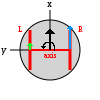
\includegraphics[width=0.15\textwidth]{robotWheels.png}
  \end{center}
  \caption{Signification physique de \(v_r,\: v_l,\: v_g \; et \; \omega_g \) \cite{argosSite1}}
  \vspace{-2em}
  \end{wrapfigure}
L'effecteur dont un footbot dispose afin de se déplacer est une paire de roues dont les vitesses peuvent être fixées de manière indépendante. A chaque instant, les seuls deux mouvements auxquels peut accéder le robot sont donc une translation parallèle aux roues et une rotation autour d'un point au milieu de l'axe des roues. La mécanique \cite{meca} nous indique que la composition de ces deux mouvements est suffisante pour permettre au robot de se déplacer librement dans un plan mais surtout, elle nous donne la relation entre les vitesses des deux roues et la vitesse générale ainsi que la vitesse de rotation du robot:
\begin{equation}
\begin{cases}
v_g=\frac{v_r+v_l}{2}\\
\omega_g=\frac{v_r-v_l}{l_{axe}}
\end{cases}  
\end{equation}

A partir de cette loi des vitesses, il est aisé de construire un algorithme permettant à un robot de converger vers sont but selon une trajectoire souple et à vitesse constante.
\begin{algorithm}                    
\caption{Convergence with no obstacle avoidance}
\label{simpleConvergence}
\begin{algorithmic}[1]
  \REQUIRE \(SPEED \equiv \) Fixed speed of the footbot \(> 0\)
  \REQUIRE Goal in arena
  \ENSURE footbot converges towards the goal at speed \(SPEED\)
  \WHILE{goal not reached}
    \STATE update footbot position and orientation
    \STATE calculate \( \theta \equiv\) angle between the direction of the goal from the footbot and footbot orientation
    \STATE \( right\:velocity \leftarrow\) convergence(\(\theta,\:SPEED\))
    \STATE \( left\:velocity \leftarrow 2 \times SPEED-right\:velocity\) \COMMENT{so that overall speed stays equal to SPEED}
    \STATE robot.wheels.set\_velocity(\(left\:velocity,\:right\:velocity\))
  \ENDWHILE
\end{algorithmic}
\end{algorithm}

Où convergence(\(\theta\), SPEED) fixe la convergence du robot vers son goal. Elle doit satisfaire:
\begin{equation}
  \begin{cases}
    convergence(0,SPEED)=SPEED\\
    convergence(\overset{\text{goal à gauche du robot}}{\overbrace{0<\theta\leq\pi}},SPEED)>SPEED\\
    convergence(\overset{\text{goal à droite du robot}}{\overbrace{0>\theta\geq-\pi}},SPEED)<SPEED
  \end{cases}
\end{equation}

Pour une fonction convergence(\(\theta, SPEED\)) donnée satisfaisant à cette condition (par exemple dépendance linéaire en \(\theta\)), le footbot peut donc se rendre d'un point A à un point B, tant qu'il ne rencontre pas d'obstacles sur son trajet. Notons que cet algorithme s'intègre particulièrement bien dans la fonction loop demandée par ARGoS. Dans notre projet nous avons choisi
\[
convergence(\theta, SPEED)=
\begin{cases}
      { \left( \frac{\pi- \lvert \theta \rvert }{\pi} \right)}^{\kappa} \times SPEED & \text{si } \theta \geq 0\\
      \left( 2 - { \left( \frac{\pi- \lvert \theta \rvert }{\pi} \right) }^{\kappa} \right) \times SPEED & \text{si } \theta < 0
\end{cases}
\]
Où $\kappa > 0$ est un paramètre qui fixe l'intensité de la convergence.

La manière la plus directe de permettre au robot d'éviter des obstacles quels qu'ils soient est d'exécuter une routine d'évitement à la place d'une routine de convergence lorsqu'un obstacle est détecté.
\begin{algorithm}                    
\caption{Convergence with obstacle avoidance}
\label{obstacleConvergence}
\begin{algorithmic}[1]
  \REQUIRE \(SPEED \equiv \) Fixed speed of the footbot \(> 0\)
  \REQUIRE goal in arena
  \ENSURE footbot converges towards the goal at speed \(SPEED\) while avoiding obstacles
  \WHILE{goal not reached}
    \STATE update footbot position and orientation
    \STATE read proximity sensors \COMMENT{or whatever other sensor in use}
    \IF{no obstacles}
      \STATE calculate \( \theta \equiv\) angle between the direction of the goal from the footbot and footbot orientation
      \STATE \( right\:velocity \leftarrow\) convergence(\(\theta,\:SPEED\))
    \ELSE
      \STATE \( right\:velocity \leftarrow\) avoidance(proximity sensor reading, \(SPEED\))
    \ENDIF
    \STATE \( left\:velocity \leftarrow 2 \times SPEED-right\:velocity\) \COMMENT{so that overall speed stays equal to SPEED}
    \STATE robot.wheels.set\_velocity(\(left\:velocity,\:right\:velocity\))
  \ENDWHILE
\end{algorithmic}
\end{algorithm}

Où avoidance(proximity sensor reading) fixe la routine d'évitement du robot. Son implémentation est très libre et peut fortement varier en fonction du capteur utilisé pour détecter les obstacles. On peut par exemple utiliser le senseur proximity du footbot, qui associe à 24 directions autour du robot une valeur entre zéro et un: une valeur zéro indique qu'aucun obstacle n'est perçu dans la direction donnée tandis qu'une valeur supérieure indique qu'un objet a été détecté. Cette valeur augmente au fur et à mesure que le robot se rapproche de l'obstacle.\cite{argosSite1} Dans notre projet nous avons choisi
\[avoidance(dir, prox)=
  \begin{cases}
      \frac{-\alpha +(1-prox)^{\beta}\cdot dir}{11}SPEED & \text{si }dir \leq 12\\
      \frac{(22+\alpha )-(1-prox)^{\beta}\cdot (25-dir)}{11}SPEED & \text{si }dir \geq 12\\
  \end{cases}
\]
Où $ 1 \leq dir \leq 12 $ est la direction de l'obstacle perçu le plus proche et \hbox{$0 \leq prox \leq 1$} donne la proximité de cette obstacle. Comme présenté plus haut, ce sont les deux informations dont on dispose si l'on utilise le capteur de proximité.  \(1 \leq \alpha \leq 12 \) est un paramètre qui fixe l'influence de la direction de l'obstacle le plus proche et \(0 \leq \beta \) fixe l'influence de la proximité de cette obstacle. Cet évitement est partiellement tiré des exemples fourni sur le site du cours présentant ARGoS \cite{argosSite1}.

Grâce à cette routine d'évitement, ainsi qu'en utilisant l'algorithme présenté plus haut, il est déjà possible de produire une solution fonctionnelle à la partie déplacement du cahier des charges, même si on peut améliorer cette solution en fonction de la connaissance de son environnement dont dispose le robot.

Ainsi, dans le cas omniscient ou si le robot est capable de construire une carte de son environnement reprenant la position des différents obstacles il peut-être judicieux d'utiliser un algorithme de recherche du plus court chemin. La manière la plus directe de faire est de donner au footbot une liste de goal successifs qui le mèneront au goal final. Ceci  permet de réutiliser facilement les algorithmes déjà présentés tout en étant parfaitement compatible avec les valeurs de retour typiques d'un algorithme de recherche du plus court chemin. En effet, la plupart des recherches du plus court chemin utilisent une représentation en graphe d'un environnement. La valeur de retour d'une telle recherche est donc une liste des nœuds qu'il faut parcourir dans le graphe afin d'arriver au but final, ce qui est précisément ce que cet algorithme fait.
\begin{algorithm}                    
\caption{Convergence with path finding}
\label{pathConvergence}
\begin{algorithmic}[1]
  \REQUIRE \(SPEED :=\) Fixed speed of the footbot \(> 0\)\\intermediate goals list := list of points which lead to the goal while avoiding the obstacles\\goal in arena
  \ENSURE footbot converges towards the goal at speed \(SPEED\) while avoiding obstacles
  \FOR{intermediate goal in intermediate goals list}
  \WHILE{goal not reached}
    \STATE update footbot position and orientation
    \STATE read proximity sensors \COMMENT{or whatever other sensor in use}
    \IF{no obstacles}
      \STATE \( \theta \leftarrow\) angle between the direction of the goal from the footbot and footbot orientation
      \STATE \( right\:velocity \leftarrow\) convergence(\(\theta,\:SPEED\))
    \ELSE
      \STATE \( right\:velocity \leftarrow\) avoidance(proximity sensor reading, \(SPEED\))
    \ENDIF
    \STATE \( left\:velocity \leftarrow 2\cdot SPEED-right\:velocity\) \COMMENT{so that overall speed stays equal to SPEED}
    \STATE robot.wheels.set\_velocity(\(left\:velocity,\:right\:velocity\))
  \ENDWHILE
  \ENDFOR
\end{algorithmic}
\end{algorithm}

L'implémentation de l'algorithme de recherche du plus court chemin qui fournit intermediate goals list est un problème à part entière. Avant de l'examiner plus en détail, il faut noter que malgré l'utilisation d'une recherche du plus court chemin qui devrait a priori permettre d'éviter les obstacles, le test d'obstacles est toujours présent, ainsi que la possibilité d'évitement. Il est évident que ceci est fait pour permettre d'éviter des objets inattendus tels que d'autres robots, par exemple. Cependant, on peut dès lors se demander s'il ne faudrait pas aussi chercher de nouveau un plus court chemin après un évitement imprévu ou si le robot a dévié d'une distance significative de sa trajectoire prévue.

\section{Recherche du plus court chemin}

\subsection{Algorithme A* \cite{wikiA*}}

En informatique, A* est un algorithme informatique qui consiste à mettre en place un processus de traçage d'un chemin traversable efficace entre des points. Les points sont considérés comme des noeuds.

A* utilise une «best-first» recherche et trouve le chemin possédant le moindre coût à partir d'un nœud initial donné à un nœud but.

Pour cela, il utilise une fonction de coût pour déterminer l'ordre dans lequel les visites de recherche des nœuds de l'arbre vont s'effectuer. Cette fonction de coût est la somme de deux autres fonctions. La fonction coût de la trajectoire passée qui est la distance connue à partir du nœud de départ au dernier parcouru lors de la recherche. Et la fonction coût du chemin futur qui est une estimation heuristique de la distance entre le dernier nœud parcouru et le nouveau nœud à atteindre .

\begin{wrapfigure}{r}{0.3\textwidth}
  \vspace{-20pt}
  \begin{center}
    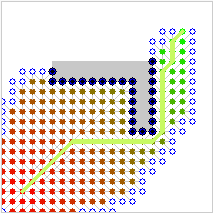
\includegraphics[width=0.28\textwidth]{aStar.png}
  \end{center}
  \caption{Représentation d'une éxécution de A*\cite{wikiA*}}
\end{wrapfigure}
Cet algorithme possède quand même des limites. Il est effectivement efficace dans le cas où l'on considère les robots comme omniscient, connaissant l'environnement et, donc, connaissant la position de la source et des obstacles se trouvant dans l'environnement. Dans le cas de non-omniscience, l'arène est inconnue et on ne possède aucunes données à propos de celles-ci. Et c'est ici que se trouve le plus grand défaut de l'algorithme A*.

A* détermine un chemin complet de nœuds pour arriver d'un noeud départ à un noeud but. Lorsqu'il ne possède pas de données complètes à propos de l'arène, il est bloqué lors de son exécution et ne peut donc pas déterminer le chemin que doit suivre le robot. Il faudra adapter l'algorithme A* afin de remédier à ce problème.

\subsection{Algoritme de Dijkstra \cite{wikiDijkstra}}

L’algorithme de Dijkstra est un algorithme servant à résoudre le problème du plus court chemin. Le principe de l'algorithme est le suivant:

Il s'agit de mettre en place progressivement un sous-graphe dans lequel sont classés les différents sommets. Un ordre croissant est établit entre les sommets et il est fixé en fonction de la distance minimale qui éloignent ces sommets à celui de départ. Cette distance correspond à la somme des nœuds parcourus.

Au début, les distances de chaque sommet par rapport au sommet de départ sont considérées comme infinie et on attribue à celui-ci une distance de 0.

Ensuite, au cours de chaque itération, les distances des sommets reliés par un nœud au dernier du sous-graphe sont mis à jour. Cette mis à jour consiste à ajouter la valeur du nœud à la distance séparant le sommet de départ à ce dernier sommet. Après cette mise à jour, l'ensemble des sommets, ne faisant pas partis du sous-graphe, sont examinés et celui qui possède la distance minimal y est ajouté.

Enfin, on répète l'exécution jusqu'à l'épuisement des sommets ou jusqu'à la sélection du sommet d'arrivée.
Voici 3 figures qui représentent un exemple du principe utilisé. Le but est de trouver le plus court chemin entre le point A et le point J. Comme dit précédemment, après chaque mise à jour, le sommet possédant la distance minimale est rajouté au sous graphe. La figure \ref{fig:dijkstra} représente bien cela.
\begin{figure}[h!]
        \centering
        \begin{subfigure}[h!]{0.4\textwidth}
                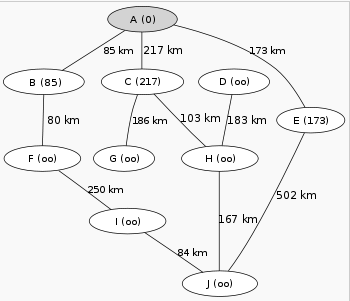
\includegraphics[width=\textwidth]{dijk1.png}
                \caption{Mise à jour initiale\\\(\;\)}
        \end{subfigure}   \begin{subfigure}[h!]{0.4\textwidth}
                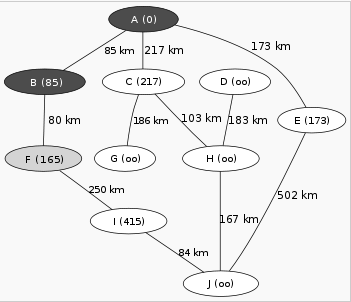
\includegraphics[width=\textwidth]{dijk2.png}
                \caption{Mise à jour et construction du sous-graphe}
        \end{subfigure}

        \begin{subfigure}[h!]{0.4\textwidth}
                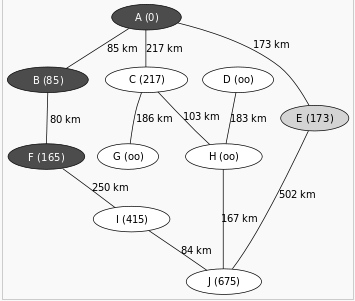
\includegraphics[width=\textwidth]{dijk3.png}
                \caption{Mise à jour et graphe final}
        \end{subfigure}
        \caption{\label{fig:dijkstra}Représentation d'une éxécution de Dijkstra \cite{wikiDijkstra}}
\end{figure}


En effet, le sommet E est rajouté au sous graphe et non le sommet I car la distance à parcourir entre A et E est plus petite que entre A et I.

Il faut souligner que cet algorithme possède le même inconvénient qu'A*.